\documentclass[border=4pt]{standalone}

\usepackage{amsmath}
\usepackage{tikz}
\usepackage{mathdots}
\usepackage{yhmath}
\usepackage{cancel}
\usepackage{color}
\usepackage{siunitx}
\usepackage{array}
\usepackage{multirow}
\usepackage{amssymb}
\usepackage{gensymb}
\usepackage{tabularx}
\usepackage{booktabs}
\usetikzlibrary{fadings}
\usetikzlibrary{patterns}


\begin{document}
 



\tikzset{every picture/.style={line width=0.75pt}} %set default line width to 0.75pt        

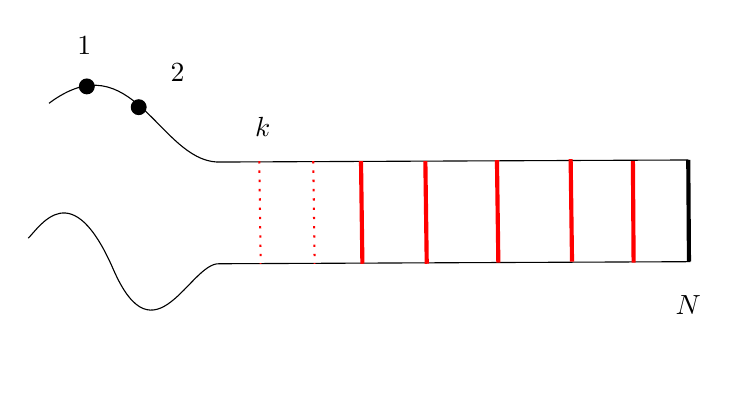
\begin{tikzpicture}[x=0.75pt,y=0.75pt,yscale=-1,xscale=1]
%uncomment if require: \path (0,300); %set diagram left start at 0, and has height of 300

%Straight Lines [id:da32105397539146907] 
\draw    (143,99) -- (370,98) ;


%Straight Lines [id:da440729150359208] 
\draw    (144,148) -- (371,147) ;


%Straight Lines [id:da11578579215087781] 
\draw [color={rgb, 255:red, 255; green, 0; blue, 0 }  ,draw opacity=1 ][line width=1.5]    (343.33,98.58) -- (343.67,147.42) ;


%Straight Lines [id:da5451435875066704] 
\draw [color={rgb, 255:red, 255; green, 0; blue, 0 }  ,draw opacity=1 ][line width=1.5]    (313.33,97.58) -- (314,147) ;


%Straight Lines [id:da8589654555416402] 
\draw [color={rgb, 255:red, 255; green, 0; blue, 0 }  ,draw opacity=1 ][line width=1.5]    (277.83,98.08) -- (278.5,147.5) ;


%Straight Lines [id:da6331312898551019] 
\draw [color={rgb, 255:red, 255; green, 0; blue, 0 }  ,draw opacity=1 ][line width=1.5]    (243.33,98.58) -- (244,148) ;


%Straight Lines [id:da2463687592245184] 
\draw [color={rgb, 255:red, 255; green, 0; blue, 0 }  ,draw opacity=1 ][line width=1.5]    (212.33,98.58) -- (213,148) ;


%Straight Lines [id:da31399629314291666] 
\draw [color={rgb, 255:red, 255; green, 0; blue, 0 }  ,draw opacity=1 ][line width=0.75]  [dash pattern={on 0.84pt off 2.51pt}]  (189.33,98.58) -- (190,148) ;


%Straight Lines [id:da12028035161596284] 
\draw [color={rgb, 255:red, 255; green, 0; blue, 0 }  ,draw opacity=1 ][line width=0.75]  [dash pattern={on 0.84pt off 2.51pt}]  (163.33,98.58) -- (164,148) ;


%Curve Lines [id:da6385422567123601] 
\draw    (62,70.7) .. controls (102,40.7) and (115,97.7) .. (143,99) ;


%Curve Lines [id:da5173143898040751] 
\draw    (52,135.7) .. controls (58,129.7) and (73,104.7) .. (93,150.7) .. controls (113,196.7) and (130,147.35) .. (144,148) ;


%Straight Lines [id:da4228517863794443] 
\draw [color={rgb, 255:red, 0; green, 0; blue, 0 }  ,draw opacity=1 ][line width=1.5]    (370,98) -- (370.34,146.84) ;


%Shape: Circle [id:dp9053423364674607] 
\draw  [color={rgb, 255:red, 0; green, 0; blue, 0 }  ,draw opacity=1 ][fill={rgb, 255:red, 0; green, 0; blue, 0 }  ,fill opacity=1 ] (76.67,62.56) .. controls (76.67,60.59) and (78.26,59) .. (80.23,59) .. controls (82.2,59) and (83.79,60.59) .. (83.79,62.56) .. controls (83.79,64.53) and (82.2,66.12) .. (80.23,66.12) .. controls (78.26,66.12) and (76.67,64.53) .. (76.67,62.56) -- cycle ;
%Shape: Circle [id:dp25543902358573356] 
\draw  [color={rgb, 255:red, 0; green, 0; blue, 0 }  ,draw opacity=1 ][fill={rgb, 255:red, 0; green, 0; blue, 0 }  ,fill opacity=1 ] (101.67,72.56) .. controls (101.67,70.59) and (103.26,69) .. (105.23,69) .. controls (107.2,69) and (108.79,70.59) .. (108.79,72.56) .. controls (108.79,74.53) and (107.2,76.12) .. (105.23,76.12) .. controls (103.26,76.12) and (101.67,74.53) .. (101.67,72.56) -- cycle ;

% Text Node
\draw (370,168) node   {$N$};
% Text Node
\draw (165,82) node   {$k$};
% Text Node
\draw (79,43) node   {$1$};
% Text Node
\draw (124,56) node   {$2$};


\end{tikzpicture}



\end{document}
